In this chapter we will give some trivial but useful lemmas for this problem.

\begin{defn}
	For any point $P\in A$ we call the set $\iT_P := \{ K \colon K\in T ,
	|KP| = \min_{i=1}^{n} |KA_i| \} $ the domain of $p$ and we call $P$
	the origin point of $\iT_{P}$.
\end{defn}	

\begin{defn}
	If $T$ and $n$ satisfies the condition in question we call the
	pair $(T, n)$  a good pair.
\end{defn}	

In this section we just consider the properties of good pairs.

\begin{lem}
	The intersection line of two adjacent domains is the perpendicular
	bisector  of the two origin points they corresponds to.
\end{lem}
This lemma can be shown by the definition of domain.

\begin{lem}
	Domains are all convex.
\end{lem}	

\begin{center}
	\begin{tikzpicture}[scale=0.8]
	
	\draw[fill][lightgray](1.91,-3.56) circle [radius=0.05];
	\draw(1.91,-3.56) circle [radius=0.05];
	\node at (2.11,-3.76) {$A_2$};
	
	
	\draw[fill][lightgray](-5,-2.42) circle [radius=0.05];
	\draw(-5,-2.42) circle [radius=0.05];
	\node at (-5.3,-2.52) {$P$};
	
	
	\draw[fill][lightgray](-1.5,-0.26) circle [radius=0.05];
	\draw(-1.5,-0.26) circle [radius=0.05];
	\node at (-1.7,-0.16) {$Q$};
	
	
	\draw[fill][lightgray](4.59,-0.28) circle [radius=0.05];
	\draw(4.59,-0.28) circle [radius=0.05];
	\node at (4.89,-0.28) {$R$};
	
	
	\draw[fill][lightgray](1.93,3.02) circle [radius=0.05];
	\draw(1.93,3.02) circle [radius=0.05];
	\node at (2.2,3.0) {$A_1$};
	
	\draw[thick][black](-5,-2.42)--(-1.5,-0.26);
	\draw[thick][black](-1.5,-0.26)--(4.59,-0.28);
	\end{tikzpicture}
\end{center}

\begin{proof}
	If $\iT_{A_1}$ is not convex, we may as well assume that $\angle PQR$
	is more than $\pi$, here $P , Q , R$ are adjacent vertexes of
	$\iT_{A_1}$. Because $T$ is convex, $PQ$ can't be the side of $T$.
	So the symmetric point of $A_1$ about $QR$ must
	be another origin point. We call it $A_2$. Since $\angle PQR > \pi$,
	the length of $|PA_1|$ is larger than $|PA_2|$. So P couldn't
	be on the side of $\iT_{A_1}$. Then we get the contradiction.
\end{proof}

There ar some lemmas about the area of each domain. For convenience,
we sometimes use $S_i$ to denote $S_{\iT_i}$,  
$S_{A_i}$ to denote $S_{\iT_{Ai}}$

\begin{lem}
	For any domain $\iT_{A_i}$ and $\epsilon > 0$, we can choose a
	point as one of points in $B$ and let the point change almost
	half area of $A$ into green. (i.e. it can change the domain
	with area at least $\frac{S_{\iT_{Ai}}}{2} - \epsilon$ into
	green.). And we can also choose two points $B_1$ and $B_2$
	so that they change almost the whole $\iT_{Ai}$ into green.
\end{lem}


\begin{center}
	\begin{tikzpicture}[scale=0.6]
	
	\draw[fill][lightgray](2.91,0.21) circle [radius=0.05];
	\draw(2.91,0.21) circle [radius=0.05];
	\draw[fill][lightgray](-0.56,5.32) circle [radius=0.05];
	\draw(-0.56,5.32) circle [radius=0.05];
	\draw[fill][lightgray](-7.49,4.44) circle [radius=0.05];
	\draw(-7.49,4.44)circle [radius=0.05];
	\draw[fill][lightgray](-9.02,-0.79) circle [radius=0.05];
	\draw(-9.02,-0.79) circle [radius=0.05];
	\draw[fill][lightgray](-7.12,-4.58) circle [radius=0.05];
	\draw(-7.12,-4.58)  circle [radius=0.05];
	\draw[fill][lightgray](0.45,-5.64) circle [radius=0.05];
	\draw(0.45,-5.64) circle [radius=0.05];
	\draw[fill][lightgray](-2.73,0.45) circle [radius=0.05];
	\draw(-2.73,0.45) circle [radius=0.05];
	\draw[fill][lightgray](-2.76,-0.20) circle [radius=0.05];
	\draw(-2.76,-0.20) circle [radius=0.05];
	\draw[fill][lightgray](-2.67,1.52) circle [radius=0.05];
	\draw(-2.67,1.52) circle [radius=0.05];
	
	\draw[thick][black](2.91,0.21)--(-0.56,5.32)--(-7.49,4.44)--(-9.02,-0.79)--(-7.12,-4.58)--(0.45,-5.64)--cycle ;
	
	\node at (-3.03,0.45) {$A_1$};
	\node at (-2.56,-0.4) {$B_1$};
	\node at (-2.47,1.76) {$B_2$};
	\node at (1.43,0.65) {$l$};
	\node at (-2.07,3.26) {$k$};
	
	\draw[dashed,thick][black](-2.34,7.46)--(-3.18,-7.94);
	\draw[dashed,thick][black](-10.45,0.87)--(5.08,0.02);
	
	\end{tikzpicture}	
\end{center}


\begin{proof}
	For any line $l$ passing through $A_1$, it divides $A$ into two parts,
	we consider the line $k$ perpendicular to $l$ and go through $A_1$. 
	
	$k$ divides $A_1$ into two parts $\iT_1$, $\iT_2$ (We assume 
	$S_1 \geq S_2 $). Let the diameter of $A_1$ be $d$, 
	choose a point $B_1$ on $k$ in $S_1$ such that 
	$|B_1A_1| \leq \frac{\epsilon}{2d}$. This 
	point meets the first requirement. Then choose another 
	point $B_2$ on $k$ in $S_2$ such that $|B_2A_1| \leq 
	\frac{\epsilon}{2d}$. The two points,  $B_1$ and $B_2$,  
	meet the second requirement.
\end{proof}

\begin{cor}
	The areas of all the domains are equal.
\end{cor}

\begin{proof}
	Suppose that $S_{A_1} \geq S_{A_2} \geq ... \geq S_{A_n}$. 
	By lemma1.3, for every $\epsilon$ we can choose two points 
	in $\iT_{A_1}$ one point in $\iT_{A_2}$ and one point in 
	$\iT_{A_3}$ ... until one point in $\iT_{A_{n-1}}$ so that 
	these points change the domain of area at least $S_{A_1} + 
	\frac{S_{A_2} + ... S_{A_{n-1}}}{2} - \epsilon $ into green.
	Then we get that $S_{A_1} + \frac{S_{A_2} + ... S_{A_{n-1}}}{2}
	- \epsilon \leq \frac{S_{A_1} + ... S_{A_n}}{2} $ is true for
	every $\epsilon$. So $S_{A_1} = S_{A_n}$, 
	we get the corollary.
\end{proof}

\begin{lem}
	Every line goes through the origin point divides the 
	domain into two parts of equal area.
\end{lem}

\begin{proof}
	Using the same notation in lemma 3, for each line passing through 
	$A_i$, choose a point $B$ which changes the area of area 
	$\frac{S_1-S_2}{2}-\epsilon$ into green and we choose other $n-1$ 
	points which change at almost half area left into green and 
	we can get that $S_1 \leq S_2$, so $S_1 = S_2$.
\end{proof}	

We can get the most useful conclusion from lemma 4.

\begin{lem}
	All the domains are centrally symmetric.
\end{lem}

\begin{center}
	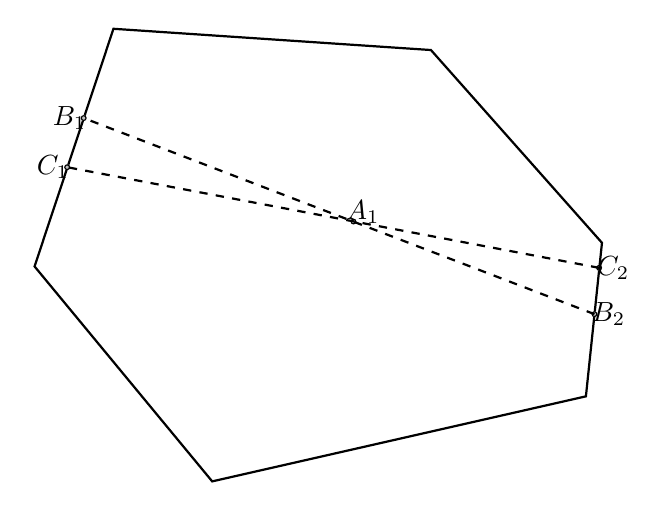
\begin{tikzpicture}[scale=0.6]
	
	\draw[thick][black](0.66,-0.24)--(-2.96,3.84)--(-9.68,4.29)
	--(-11.35,-0.74)--(-7.59,-5.29)--(0.32,-3.49)--cycle ;
	
	
	\draw[fill][lightgray](0.6,-0.77) circle [radius=0.05];
	\draw(0.6,-0.77) circle [radius=0.05];
	\draw[fill][lightgray](0.5,-1.75) circle [radius=0.05];
	\draw(0.5,-1.75) circle [radius=0.05];
	\draw[fill][lightgray](-4.6,0.21) circle [radius=0.05];
	\draw(-4.6,0.21) circle [radius=0.05];
	\draw[fill][lightgray](-10.31,2.4) circle [radius=0.05];
	\draw(-10.31,2.4) circle [radius=0.05];
	\draw[fill][lightgray](-10.66,1.36) circle [radius=0.05];
	\draw(-10.66,1.36) circle [radius=0.05];
	
	\node at (0.9,-0.77) {$C_2$};
	\node at (0.8,-1.75) {$B_2$};
	\node at (-4.4,0.41) {$A_1$};
	\node at (-10.61,2.4) {$B_1$};
	\node at (-10.96,1.36) {$C_1$};
	
	\draw[dashed,thick][black](0.5,-1.75)--(-10.31,2.4);
	\draw[dashed,thick][black](0.6,-0.77)--(-10.66,1.36);
	
	\end{tikzpicture}	
\end{center}


\begin{proof}
	For each line passing through $A_1$, it intersects the boundary 
	of the domain at two points $B_1$ and $B_2$. If $|A_1B_1| > |A_2B_2|$, 
	we rotate the line  by  a small angle $\theta$ and let the two new 
	points of intersection $C_1$ and $C_2$ satisfies $|A_1C_1| \geq |A_2C_2|$. 
	Then we know  $S_{A_1B_1C_1} = \frac{1}{2}|A_1B_1||A_1C_1|sin\theta >  \frac{1}{2}|A_1B_2||A_1C_2|sin\theta = S_{A_1B_2C_2}$. From lemma 4
	$S_{A_1B_1C_1}=S_{A_1B_2C_2}$, then we get the 
	contradiction. So $|A_1B_1|=|A_2B_2|$ for any line, 
	which implies that $\iT_{A_1}$ is centrally symmetric
\end{proof}

Now we have gotten all tools we need and then discuss an example
to use these tools.
